%% Template for MLP Coursework 3

%% Based on  LaTeX template for ICML 2017 - example_paper.tex at 
%%  https://2017.icml.cc/Conferences/2017/StyleAuthorInstructions
\documentclass{article}
\usepackage[T1]{fontenc}
\usepackage{amssymb,amsmath}
\usepackage{txfonts}
\usepackage{microtype}
\usepackage{xspace}
\xspaceaddexceptions{\%}

% Lists with less spacoing between items
\usepackage{paralist}

% For figures
\usepackage{graphicx}
\usepackage{subfig} 

% For citations
\usepackage{natbib}

% For algorithms
\usepackage{algorithm}
\usepackage{algorithmic}

% the hyperref package is used to produce hyperlinks in the
% resulting PDF.  If this breaks your system, please commend out the
% following usepackage line and replace \usepackage{mlp2017} with
% \usepackage[nohyperref]{mlp2017} below.
\usepackage[hyphens]{url}
\urlstyle{same}
\usepackage{hyperref}

% Packages hyperref and algorithmic misbehave sometimes.  We can fix
% this with the following command.
\newcommand{\theHalgorithm}{\arabic{algorithm}}


% Set up MLP coursework style (based on ICML style)
\usepackage{mlp2020}
\mlptitlerunning{MLP Coursework 4 -- Final Report (\groupNumber)}
\bibliographystyle{icml2017}


\DeclareMathOperator{\softmax}{softmax}
\DeclareMathOperator{\sigmoid}{sigmoid}
\DeclareMathOperator{\sgn}{sgn}
\DeclareMathOperator{\relu}{relu}
\DeclareMathOperator{\lrelu}{lrelu}
\DeclareMathOperator{\elu}{elu}
\DeclareMathOperator{\selu}{selu}
\DeclareMathOperator{\maxout}{maxout}







%% You probably do not need to change anything above this comment

%% REPLACE this with your project title, group ID and list of student numbers for the group
\def\projectTitle{Title}
\def\groupNumber{G125}
\def\studentNumbers{s1765263, s1645474, s2067275}
\usepackage{tabularx}
\usepackage{graphics}
\newcolumntype{Y}{>{\centering\arraybackslash}X}
\usepackage{multirow}
\usepackage[dvipsnames]{xcolor}
\usepackage[table]{xcolor}
\usepackage{xcolor}

\begin{document} 

\twocolumn[
\mlptitle{ Illuminating Zelda Rooms in the Latent Space of a Deep Convolutional Generative Adversarial Network}

\centerline{\groupNumber\ (\studentNumbers)}

\vskip 7mm
]

\begin{abstract} 
% The abstract should be a few sentences (100--200 words) long,  providing a concise summary of the contents of your report including the key research question(s) addressed, the methods explored, the data used, and the findings of the experiments.
Generative Adversarial Networks (GANs) are now powerful and popular tools for the task of content generation, but are not free from downsides. Generated content may be missing certain important qualities and can be lacking in diversity when training data is scarce. When paired with quality diversity techniques such as Covariance Matrix Adaptation MAP-Elites (CMA-ME), generative adversarial networks capably generate synthetic content that is not only high-quality but also diverse. Here, we apply this technique to the generation of playable levels for \textit{The Legend of Zelda} by exploring the latent space of the generative network in terms of the level characteristics produced. We compare the resulting rooms generated to those generated via other methods in terms of diversity of environment. We also use a Zelda-playing agent to optimise for completability of rooms generated and compare the generation methods further. We find that the MAP-Elites algorithm represents a significant improvement in terms of both completability and diversity of rooms generated over a random search of the GAN latent space. We also find that CMA-ME in turn represents a significant improvement over MAP-Elites in terms of diversity without comprimising on completability.


\end{abstract} 

\section{Introduction}
\label{sec:intro}
% This document provides a template for the MLP coursework 3 interim report.  This template structures the report into sections, which you may use,or you can structure it differently if you wish.  If you want to use subsections within a section that is fine. In this template the text in each section will include a very brief outline of what you should include in each section, along with some practical LaTeX examples (for example figures, tables, algorithms).  Your document should be no longer than \textbf{five pages},  with an additional page (or more!) allowed for references.

% You should give a broad introduction to the project, including citations to related work. Your aim here is to explain why the project is addressing an interesting topic, and how it relates to things that have been done in the area.

% You should make clear what are the aims and objectives of the project, what are the research questions being addressed.  Be precise. In this section you should make clear what the project's contribution is: how is it different to what is already done. 

% The interim report should state the objectives of the project, which are related to the research questions. What experiments do you plan to carry out? You can differentiate between core objectives, and optional objectives you hope to achieve if things go well. The conclusions in your final report should relate to these objectives.

% Use bibtex to organise your references -- in this case the references are in the file \verb+example-refs.bib+.  Here is a an example reference \citep{langley00}.  

Generative adversarial networks (GANs) \cite{Goodfellow2014} represent a versatile tool for computer generation of content, and have been applied to many areas, such as the ones mentioned in \cite{Banjo2020,Antipoy2017,Paganini2018,Lan2020}. However, while GANs can often learn to produce high-standard imitations of given content, they don't necessarily generalise to a diverse distribution of these imitations when given limited datasets. Nor do they necessarily produce content with particular desirable qualities which may be no trouble for alternative, more heavily scripted content generation algorithms. Previous attempts have been made to `steer' GANs in a particular direction with respect to certain qualities of the generated output - such as rotation and scale of objects in generated pictures \cite{Jahanian2019} - by manipulating the GAN's latent space. While impressive, these approaches are limited and require training of an additional algorithm.

Quality diversity algorithms (QD) provide a promising path around the diversity problem. They seek to ensure, for a given search space, that not only are returned solutions high quality with respect to a given objective function, but that a diverse range of such solutions is returned. One such approach to QD is illumination: choosing meaningful dimensions along which to stratify the search space, performing a genetic-algorithm-style search, and recording the individuals from each strata with the highest score on the objective \cite{Mouret2015}. This can be applied to the latent space of a GAN in order to identify latent vectors that produce certain qualities in the generated output \cite{Fontaine2020}.

Video games provide a fantastic context for testing algorithms in general due to their often predictable dynamics, low-noise outputs and intuitive digital representations. One particular area of interest in video game AI is procedural content generation (PCG) - many games involve partially or fully computer-generated environments/characters. However, PCG for video game levels can be a balancing act between ensuring playability and giving the algorithm creative freedom.

Here, we present an illuminated GAN as a method for generating \textit{The Legend of Zelda (1986)} levels. Using a GAN rather than an algorithm with a hard-coded completability constraint, as well as applying illumination should guarantee a diverse range of generated levels that make use of a larger share of the search space - usually a desirable quality in video game levels and much other content. Our method follows previous work which took a similar approach to \textit{Super Mario Bros (1985)} \cite{Fontaine2020}. We seek in particular to generate levels which pose diverse challenges to the player, for example varying the enemies fought and the length of time required to progress during each level. We will also evaluate these generated levels in terms of their completability using an A* agent.

This paper is structured as follows: Section 2 describes the dataset we use and how we evaluate it; Section 3 concerns the models and algorithms used; Section 4 details the experiments we carried out; Section 5 discussed related research; and Section 6 evaluates our work and discusses future work on this topic.


\section{Data Set and Task} 
% Clearly describe the data set and task you will be exploring.  If the data requires any preprocessing, then explain this.  The description should be in enough detail such that your work would be reproducible by another group.  Describe how you will evaluate the task (for example, classification accuracy).  Use citations where appropriate.
\subsection{Data}
The Legend of Zelda as a game is made up of an overworld and levels. The levels are subdivided into rooms, each taking the space of a single screen, with only one room shown to the player at a time. A room may contain anything from Table \ref{table:tiles}, but must contain at least a single entry or exit point. The game contains 9 individual levels with a total of 237 screens.

To access the individual rooms, data was pulled from the The Video Game Level Corpus (VGLC) \cite{schrum2020}. In this repository, each room in game's levels has been saved as an txt file with tiles encoded into different characters in a 11 x 16 grid. Before the data is input into the GAN, the txt file is converted into a 2D array and characters are encoded once again into numbers. It is then padded with void tiles to be square and turned into a 3D array of one-hot encodings of shape 14 x 16 x 16. Some rooms contain tiles not described in the VGLC documentation and which are not present in the full levels. In practice these were rare enough to be ignored and we theorise that they correspond to the starting locations of Link and bosses.

 

\begin{table}
\begin{center}
    \begin{tabularx}{\columnwidth}{Y|Y|Y|Y}
         \hline
         Tiles & Encoded Tiles (Characters) & Encoded Tiles (Numbers) & Graphic \\ \hline
         Void & - & 0 & \includegraphics{0.png}\\
         Wall & W & 1 & \includegraphics{1.png}\\
         Floor & F & 2 & \includegraphics{2.png}\\
         Block & B & 3 & \includegraphics{3.png}\\
         Monster & M & 4 & \includegraphics{4.png}\\
         Element (Lava, Water) & P & 5 & \includegraphics{5.png}\\
         Element + Floor & O & 6 & \includegraphics{6.png}\\
         Element + Block & I & 7 & \includegraphics{7.png}\\
         Door & D & 8 & 
\includegraphics{8.png}\\
         Stair & S & 9 & 
\includegraphics{9.png}\\
         \hline
    \end{tabularx}
\end{center}
\caption{Encoding details of the tiles in Zelda excluding the 4 unknown tiles}
\label{table:tiles}
\end{table}

\subsection{Evaluating Rooms}
With the rooms used as training data, our goal is to train a generator that is able to generate Zelda room that are indistinguishable from the rooms given as training data. After we have a generator that is capable of the above task, we will apply the illumination methods MAP-Elites and CMA-ME to the generator, in order to obtain diverse sets of rooms.

To evaluate the rooms generated, two metrics were used. First is to see if the room is completable.  To do this, we use an run basic checks such as ensuring there are at least two doors in the room. Then an A* agent is used to find a path between the doors if possible, possibly defeating monsters on the way. The second metric is the average L2 similarity between the rooms generated and all the training rooms in their 3D one-hot array form. 
\begin{center}
\Large
$L_2(X, Y) = \sqrt{\sum\limits_{i=1}^{n} (X_i - Y_i)^2}$\\\vspace{3mm}
\footnotesize
$X_i$ and $Y_i$ are components of vector X and Y respectively 
\end{center}

\subsection{Evaluating Illumination Methods}
An illumination method is successful if it produces diverse and high quality outputs. Thus we evaluate MAP-Elites and CMA-ME by: the number of rooms with unique sets of characteristics they generate; the percentage of these rooms that are completed by our agent; and the percentage of the possible space of certain characteristics that they utilise. These metrics will be discussed in further detail in Section 4.2, as it is beneficial to have read section 3 beforehand.


\section{Methodology}
\subsection{Generative Adversarial Network}
Generative Adversarial Networks were introduced by \cite{Goodfellow2014}. A generator network G, and a discriminator D will be trained at the same time. Generator G takes in a random vector and will generate a room from that vector. Discriminator D will take rooms from the original game and from G, and will try to distinguish which are real and which are fake. These two models will essentially compete against one another, the discriminator D aims to minimize the probability of miss judgement, while generator G aims to maximize that probability. The generator G's training is complete when it can steadily generates rooms that causes D to have the same accuracy as a random classifier.

\begin{figure}[tb]
\vskip 5mm
\begin{center}
\centerline{\includegraphics[width=\columnwidth]{DCGAN}}
\caption{DCGAN architecture}
\label{fig:dcgan}
\end{center}
\vskip -5mm
\end{figure} 
\subsection{GAN Models}

Deep Convolutional Neural Networks are used to train both the generator and discriminator, the architecture of the network is shown in figure \ref{fig:dcgan} . For the generator it receives a latent vector of size 16 and will pass it through the convolution layers until a 10 x 16 x 16 matrix is generated. The discriminator receives a 10 x 16 x 16 matrix and will pass it through the convolution layers producing a vector of size 1, which indicates whether the room is from the original game or not. The model uses strided convolutions in the discriminator and fractional-strided convolutions in the generator. Batchnorm are used in both the models after every layer. ReLU activation are used in all layers of the generator where LeakyReLU activation are used in the discriminator. %Is part of this just copied and pasted from Fontaine? Need to reword a little if it is.

After training the GAN, the generator would be able to generate a 10 x 16 x 16 matrices, and we would combine the 10 channels back into one channel resulting with a 16 x 16 matrix, then we would crop away the bottom 5 rows of the room resulting with a 11 x 16 room.

\subsection{Quality Diversity Algorithms}
Quality diversity algorithms - presented by \cite{Gravina2019} - are a set of algorithms which seek to generate a diverse set of high quality solutions. In terms of Zelda room generation, the goal of a QD algorithm is to search for rooms that the GAN generates.

The generator of the GAN generates each room from a latent vector it takes as input in a deterministic but not human-predictable manner. Using a QD algorithm allows us to search the latent vector space for specific features in the output space.

\subsection{Illumination}
The Multi-dimensional Archive of Phenotypic Elites (MAP-Elites) algorithm \cite{Mouret2015} is an example of QD. First, the user chooses several important characteristics which they seek variety within - these are called behavioural characteristics (BCs). Illumination methods are QDs which use BCs, such as MAP-Elites. Together the BCs form a behavior space and this space is tessellated into hypervolumes. An evolutionary algorithm is used to generate a population of individual samples via mutation operations from an initial random population. We keep track of which individual has the highest fitness or performance within individuals that fall into the same BC hypervolume and call this individual the elite. Once a sufficient number of these hypervolumes are occupied by an elite, or once another termination condition is met, MAP-Elites returns the elite individuals.

\begin{algorithm}[ht]
\begin{algorithmic}
   \STATE X = \{\}, P = \{\}
   \FOR {$i=1$ {\bfseries to} max\_iter}
   \IF{$i < population\_size$} 
   \STATE $x = get\_random\_solution()$
   \ELSE
   \STATE $x' = random\_choice(X)$
   \STATE $x = variation(x')$
   \ENDIF
   \STATE $b = feature\_descriptor(x)$
   \STATE $p = performance(x)$
   \IF {$b$ {\bfseries not in} $X$ {\bfseries or} $p > P[b]$}
   \STATE $X[b] = x$
   \STATE $P[b] = p$
   \ENDIF
   \ENDFOR
   \RETURN X, P
\end{algorithmic}
  \caption{MAP-Elites}
  \label{alg:example}
\end{algorithm}

Covariance Matrix Adaptation MAP-Elites (CMA-ME) is an improvement upon MAP-Elites, which uses Covariance Matrix Adaptation Evolution Strategy (CMA-ES), an evolutionary algorithm for optimising a search. CMA-ME maintains different so-called emitters, which are analogous to CMA-ES instances. The emitters will rank solutions higher if they fill previously unfilled cells, other solutions are ranked on their improvement on the fitness of the current cells. Thus CMA-ME is driven towards engaging in greater exploration of the behaviour space than MAP-Elites.


\subsection{The Agent}
Originally we planned on using an agent trained using deep reinforcement learning \cite{torrado2018deep} on the General Video Game AI (GVGAI) framework. Unfortunately we ran in to compatibility issues with various required packages and so instead we built an A*.

We will briefly explain how we apply the A* search algorithm to our problem. This search algorithm treats every tile in the room as a node, with adjacent tiles treated as child nodes. Only reachable tiles will be considered - i.e. floor tiles and the monster tiles (as you can defeat the monster and walk through it). Next, the agent will pick the child node with the lowest cost, which is estimated by $f(n) = g(n) + h(n)$, where $f(n)$ is the cost, $g(n)$ is the cost from current node to this child node and $h(n)$ is a heuristic function that estimates the cost of the path from the child node to the goal. The above process is repeated until the goal is reached. 

A major advantage of using the A* agent is that it is always guaranteed to find a path where possible and will return the shortest path available. The downside is that the agent we implemented is only a path finding agent instead of an agent that actually understand and plays the game like the GVGAI agent mentioned above. Because of this our agent is limited to collecting simple data for evaluations such as the number of enemies beaten and the number of steps it took to clear the room. 
%\label{sec:expts}
%TODO
% The interim report should include some experimental results.  In most cases these will be baseline experiments.  Baseline experiments refer to experiments conducted using well-understood approaches against which you can compare later results.  For example if you were exploring a new data set, the baselines might include linear networks and deep neural networks with different numbers of hidden layers;  if you were exploring a different approach to regularisation, then the baselines would include no regularisation, and conventional techniques such as L1, L2, and dropout.  You can include the results of any further experiments in your interim report.

% Present the experimental results clearly and concisely.  Usually a result is in comparison or contrast to a result from another approach please make sure that these comparisons/contrasts are clearly presented.  You can facilitate comparisons either using graphs with multiple curves or (if appropriate, e.g. for accuracies) a results table. You need to avoid having too many figures, poorly labelled graphs, and graphs which should be comparable but which use different axis scales. A good presentation will enable the reader to compare trends in the same graph -- each graph should summarise the results relating to a particular research (sub)question.

% There is no need to include code or specific details about the compute environment.

% As before, your experimental sections should include graphs (for instance, figure~\ref{fig:sample-graph}) and/or tables (for instance, table~\ref{tab:sample-table})\footnote{These examples were taken from the ICML template paper.}, using the \verb+figure+ and \verb+table+ environments, in which you use \verb+\includegraphics+ to include an image (pdf, png, or jpg formats).  Please export graphs as 
% \href{https://en.wikipedia.org/wiki/Vector_graphics}{vector graphics}
% rather than \href{https://en.wikipedia.org/wiki/Raster_graphics}{raster
% files} as this will make sure all detail in the plot is visible.
% Matplotlib supports saving high quality figures in a wide range of
% common image formats using the
% \href{http://matplotlib.org/api/pyplot_api.html\#matplotlib.pyplot.savefig}{\texttt{savefig}}
% function. \textbf{You should use \texttt{savefig} rather than copying
% the screen-resolution raster images outputted in the notebook.} An
% example of using \texttt{savefig} to save a figure as a PDF file (which
% can be included as graphics in a \LaTeX document is given in the coursework document.

% If you need a figure or table to stretch across two columns use the \verb+figure*+ or \verb+table*+ environment instead of the \verb+figure+ or \verb+table+ environment.  Use the \verb+subfigure+ environment if you want to include multiple graphics in a single figure.

% \begin{figure}[tb]
% \vskip 5mm
% \begin{center}
% \centerline{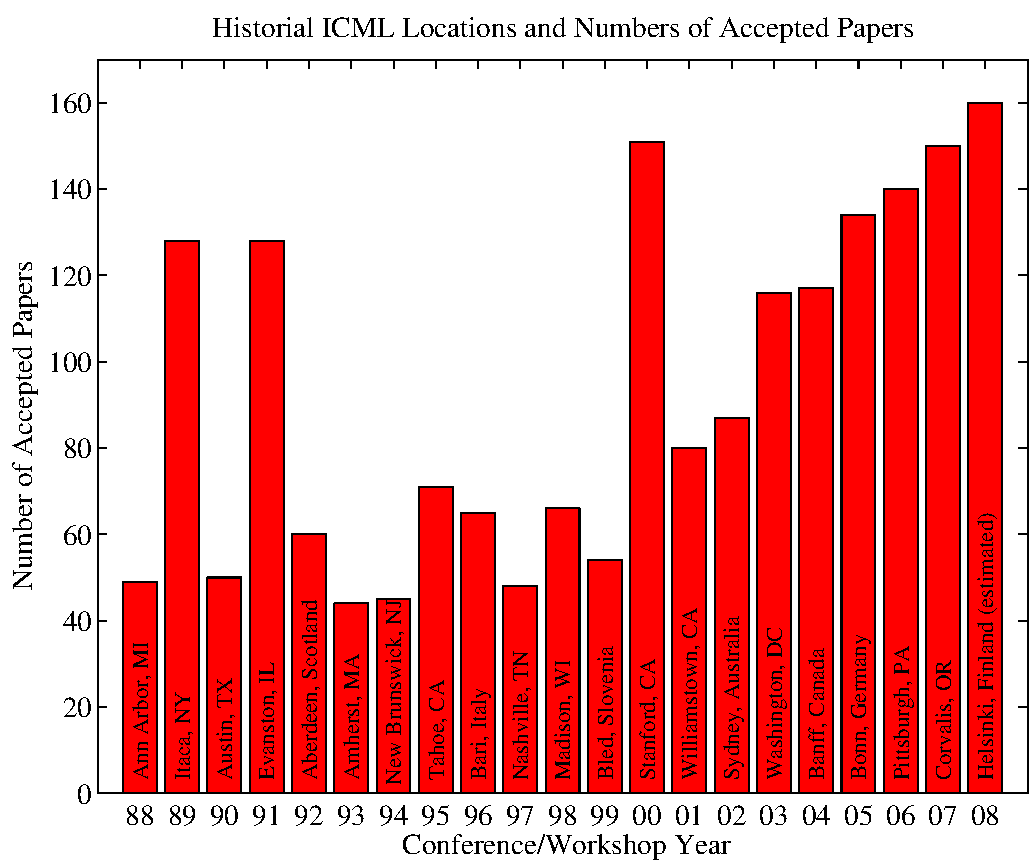
\includegraphics[width=\columnwidth]{icml_numpapers}}
% \caption{Historical locations and number of accepted papers for International
%   Machine Learning Conferences (ICML 1993 -- ICML 2008) and
%   International Workshops on Machine Learning (ML 1988 -- ML
%   1992). At the time this figure was produced, the number of
%   accepted papers for ICML 2008 was unknown and instead estimated.}
% \label{fig:sample-graph}
% \end{center}
% \vskip -5mm
% \end{figure} 

% \begin{table}[tb]
% \vskip 3mm
% \begin{center}
% \begin{small}
% \begin{sc}
% \begin{tabular}{lcccr}
% \hline
% \abovespace\belowspace
% Data set & Naive & Flexible & Better? \\
% \hline
% \abovespace
% Breast    & 95.9$\pm$ 0.2& 96.7$\pm$ 0.2& $\surd$ \\
% Cleveland & 83.3$\pm$ 0.6& 80.0$\pm$ 0.6& $\times$\\
% Glass2    & 61.9$\pm$ 1.4& 83.8$\pm$ 0.7& $\surd$ \\
% Credit    & 74.8$\pm$ 0.5& 78.3$\pm$ 0.6&         \\
% Horse     & 73.3$\pm$ 0.9& 69.7$\pm$ 1.0& $\times$\\
% Meta      & 67.1$\pm$ 0.6& 76.5$\pm$ 0.5& $\surd$ \\
% Pima      & 75.1$\pm$ 0.6& 73.9$\pm$ 0.5&         \\
% \belowspace
% Vehicle   & 44.9$\pm$ 0.6& 61.5$\pm$ 0.4& $\surd$ \\
% \hline
% \end{tabular}
% \end{sc}
% \end{small}
% \caption{Classification accuracies for naive Bayes and flexible 
% Bayes on various data sets.}
% \label{tab:sample-table}
% \end{center}
% \vskip -3mm
% \end{table}











% \section{Plan ---> Experiments?}
% \label{sec:plan}
% % Based on what you have done so far, present a plan for the rest of the project.  Are there any changes to the objectives?  What are the risks?  Do you need a backup plan?
% We plan to generate Zelda rooms using a GAN - without any QD - with the same structure as that used in prior work, as previously mentioned. This will act as a baseline to sample rooms from and can be used to measure how much of the BC space would be utilised given no specific attempt to do so.

% We will then implement a similar GAN which does employ QD, again largely following previous work such as \cite{Fontaine2020}, and report on its performance on the Zelda domain. We will compare and contrast the diversity - in terms of metrics we design for Zelda levels - between the baseline GAN and GANs which utilise QD methods.

% We may also make attempts to optimise the structure of the GAN specifically to the task of generating Zelda levels. Although this does not relate directly to level diversity, it may aid future comparisons between this work and other work which seeks to generate Zelda levels by different means, such as \cite{justesen2018}.

% If time permits, we may attempt to assemble generated levels into larger 'worlds', within which individual levels must be navigated, sometimes sequentially, to reach a final destination. This could be done using a graph representation of the larger world with each individual level being a node of the graph, à la \cite{gutierrez2020}. This would present additional challenges, as it allows for doors in one level to require a key from another level to unlock. This would relate to our objectives as it may be possible to, given a graph with specifications for attributes possessed by nodes - such as presence of a key - search for levels which posses these attributes by defining them as the BCs that illumination should select for. This would require some modification to the training set.

\section{Experiments}
%\subsection{Without Illumination}
This project is available on Github.
\footnote{https://github.com/1645474/ZeldaGAN-LSI}
\subsection{Training}

As discussed previously, our neural net design followed that of \cite{Fontaine2020} and \cite{Volz2018} and as such we used similar hyperparameters for training. In particular we used a learning rate of $5 \times 10^{-5}$ for both the generator and discriminator networks; a batch size of 32; RMSProp as our optimisation method; and trained for 5000 epochs. Our latent space was only 16-dimensional, compared to \cite{Fontaine2020}'s 32 dimensions. This is because Zelda rooms contain fewer distinct tile types and each room is smaller than a Mario level section generated by their network.

We trained using these setting with three different seeds and found the results to be easily satisfactory enough - in terms of completability and L2 distance of rooms - to apply illumination.


\subsection{Behavioral Characteristics and Coverage}

\begin{table*}
\begin{center}
\small
    \begin{tabular}{c|c|c|c}
         \hline
         Name & Type & Range & Description\\ \hline
         Steps & Discretised & 0-8 & a measure of how many tiles the agent had to traverse to complete the room, or 0 if it couldn't \\
         Kills & Literal & 0-8 & how many enemies the agent killed while completing the room\\
         Enemies & Literal & 0-8 & total number of enemies present in the room\\
         Blocks & Discretised & 0-8 & a measure of how many block tiles were present in the room\\
         Water & Discretised & 0-8 & a measure of how many water tiles were present in the room \\
         L2 & Binary & 0-1 & whether the mean L2 distance from the training rooms is greater than 8.61\\
         \hline
    \end{tabular}
\end{center}
\caption{Behavioural Characteristics for the MAP-Elite Algorithm}
\label{table:bcs}
\end{table*}

We chose the room properties as detailed in \ref{table:bcs} as our behavioural characteristics for illumination. `Steps' and `Kills' are obvious metrics for determining how a room feels to play and ones we would like to see significant variation in; if these metrics are low, the room will likely be too simple to be entertaining; too high and the room may be too difficult, especially for new players. These metrics are measured by our agent and do not cover every possible solution to each room, only a relatively short one. Through experimentation on generated rooms it was determined that the absolute number of steps to complete a room never exceeded 40. The same was true of the original training rooms. We discretised this range into 9 buckets: if a room was uncompletable its `Steps' characteristic was 0, otherwise its `Steps' characteristic was given by $ceiling($number of steps to complete room$ / 5)$. This approach makes more sense than using the exact number of steps to complete the room because the exact number is not very important to the room design; it is, however, typical for games to divide their levels into difficulty brackets 

`Enemies' and `Blocks' and `Water' are simple characteristics which describe the makeup of a room. We observed that the natural range of number of enemies in generated rooms did not exceed 8. For the other two characteristics we used a similar discretisation approach as for `Steps'.

We calculated the mean L2 distance between the training rooms to be 6.81. Our `L2' characteristic therefore tells us whether the generated room is a greater or lesser L2 distance from the training rooms' average than they were.

To measure the exploration of the algorithms examined, we use a metric which we call `W/B/E Coverage'. This metric attempts to estimate the percentage of the possible rooms - described in terms of Water, Blocks and Enemies - which the algorithm generated. Due to our discretisation of the BCs, the number of possible rooms is extremely difficult to accurately calculate given how the number of blocks, water tiles and enemies are related to each other. Therefore we estimate the number of possible BC combinations by multiplying the number of values explored across all generated and training rooms for each BC, yielding 2106. We note that this number includes impossible rooms - i.e. ones containing more than 84 tiles - and excludes possible rooms (although most of these would be uncompletable). For reference, 24 different W/B/C combinations are present in the training rooms from the original game which would give a W/B/C coverage of 1.14\%. There are only 237 such rooms however, and as such this percentage should not be compared directly to those obtained during our experiments which generated far more rooms. Steps and Kills are unused for this metric as, by design, our agent finds the simplest path through each room and as such provides little information about the range of total possibilities of room architecture.
%For example, on one room from the original game which contains 12 enemies the agent will only ever kill one

\subsection{Random Generation}

As a baseline comparison we performed three runs of generating 10000 samples without any kind of illumination method. The latent vectors for these samples were generated from a Gaussian distribution with mean 0 and variance 1. These samples were then classified by their behavioural characteristics so as to have a set with unique characteristics comparable to the set of elites generated by the other two methods.

\subsection{Map-Elites Performance}

We ran the standard MAP-Elites algorithm using the behavioural characteristics and model described above. The algorithm was run until 10000 individuals had been generated and evaluated. This experiment was repeated three times with different initial populations to reduce the risk of anomalous behaviour. The results are shown in table \ref{table: results}.

Compared to the random baseline, MAP-Elites generated significantly more rooms with unique combinations of the BCs (705 vs. 988) and a higher percentage of possible rooms were explored (7.68\% vs 8.51\%). Furthermore, a higher percentage of the rooms generated were completable (71.12\% vs. 77.69\%). This higher completion rate is to be expected as the latent vectors for MAP-Elites are created from previously generated elites which are themselves more likely to be completable than the average randomly generated room as completability is used as the fitness metric.




\subsection{CMA-ME Performance}

We ran CMA-ME using the behavioural characteristics and model described above. similarly to MAP-Elites, the algorithm was run until 10000 individuals had been generated and evaluated with this process being repeated three times. The results are shown in table \ref{table: results}.

CMA-ME achieved better results across the board than both the baseline and MAP-Elites: all of the best values obtained occurred when on CMA-ME runs and the CMA-ME mean values were superior to the mean values for the other methods. The gains made by CMA-ME over MAP-Elites for the number of elites generated and W/B/E coverage are comparable to those of MAP-Elites over the random baseline - i.e. CMA-ME is a very significant improvement. This indicates that the measures employed by CMA-ME based on CMA-ES to boost exploration are working effectively and the fact we also saw an increase in completability suggests this exploration didn't come at the cost of another desirable trait.



\begin{table*}
\begin{center}
\small
    \begin{tabular}{|c|c|c|c|c|c|c|c|c|c|c|c|c|}
        \hline
        \multirow{2}{*}{Method} 
        & \multicolumn{4}{c|}{Random} 
          & \multicolumn{4}{c|}{MAP-Elites} 
            & \multicolumn{4}{c|}{CMA-ME}\\  
                    \cline{2-13}
            & 1 & 2 & 3 & \textbf{Mean} & 1 & 2 & 3 & \textbf{Mean} & 1 & 2 & 3 & \textbf{Mean} \\
        \hline
        Elites Generated & 714 & 712 & 691 & \textbf{705.67} & 951 & 960 & 1053 & \textbf{988} & \color{YellowGreen}{1213} & 1044 & 1108 & \textbf{1121.67}\\
        \hline
        Completable Elites & 512 & 508 & 486 & \textbf{502} & 736 & 736 & 832 & \textbf{768} & \color{YellowGreen}{946} & 808 & 832 & \textbf{862}\\ 
        \hline
        Completability (\%) & 71.67 & 71.35 & 70.33 & \textbf{71.12} & 77.39 & 76.67 & 79.01 & \textbf{77.69} & 77.99 & 77.39 & \color{YellowGreen}{79.51} & \textbf{78.30}\\
        \hline
        W/B/E Coverage (\%) & 7.69 & 7.74 & 7.60 & \textbf{7.68} & 8.45 & 8.31 & 8.78 & \textbf{8.51} & \color{YellowGreen}{9.97} & 9.35 & 9.16 & \textbf{9.50}\\
        \hline
    \end{tabular}
\end{center}
\caption{Results of the three elite generation methods. All figures rounded (if applicable) to two decimal places.}
\label{table: results}
\end{table*}

\subsection{Generated Rooms}


As well as any effects on exploration and completability, another advantage of using an elites-based method is that we are provided with a list of elite rooms broken down by behaviour characteristics; thus we can chose any type of room that takes the player's fancy by its properties. For example, we could chose a room with the highest Water characteristic of any generated room but no blocks or enemies \ref{level 30}. Rooms with more extreme BC values tend to have higher L2 values and look less like human-designed rooms. However, high L2 rooms, while less conventional, are are often still completable - 79.92\% of the time for CMA-ME for instance. For example, the room shown in \ref{level longest}, which had the largest Steps characteristic and even contains a void tile in the middle of the room.

Full levels in the original game often contain more complex objectives, such as obtaining a key in one room to unlock a locked door in another. Some generated rooms appear to be far too easy, but may be based on patterns present in rooms which would normally contain such additional objectives. For example, the addition of a key to the top-right area of \ref{additional mechanics} would make for a room which forces the player to walk past enemies which then corner them between blocks and walls.

Where generated rooms fail to be completable they are often not far off. A common problem is the presence of only one door for example. Many such problems could be easily fixed by a hard-coded program after generation if these level-generation techniques where to be used in a practical application. For example a script which detected when a block tile was obstructing a door tile and removed it would turn \ref{broken} into a challenging but legitimate room.


\begin{figure}
    \centering
    \includegraphics[width=\linewidth]{Level 30 No Blocks Water Level.png}
    \caption{(MAP-Elites generated) A completable elite with zero enemies or blocks and a water level of seven.}
    \label{level 30}
\end{figure}

\begin{figure}
    \centering
    \includegraphics[width=\linewidth]{longest_path.png}
    \caption{(MAP-Elites generated) A high L2 room with Step = 8.}
    \label{level longest}
\end{figure}

\begin{figure}
    \centering
    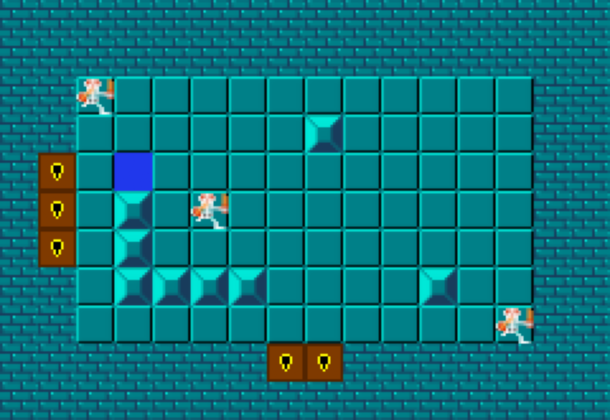
\includegraphics[width=\linewidth]{CMAME 9100 Boring.png}
    \caption{(CMA-ME generated).}
    \label{additional mechanics}
\end{figure}

\begin{figure}
    \centering
    \includegraphics[width=\linewidth]{8195 Busy and Good.png}
    \caption{(CMA-ME generated) A slightly invalid room.}
    \label{broken}
\end{figure}

\begin{figure}
    \centering
    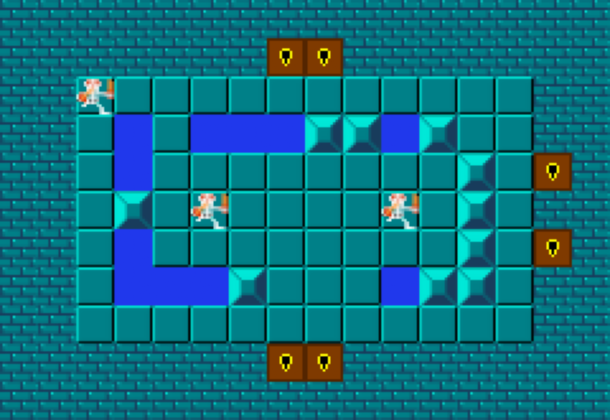
\includegraphics[width=\linewidth]{CMAME 1 9183 Busy but good.png}
    \caption{(CMA-ME generated) A room which uses several of each B/W/E tile type.}
    \label{b/w/e}
\end{figure}






\section{Related Work}
The key concept for our experiment, illumination, was first proposed by \cite{Mouret2015}. They used illumination to to perform searches in three different spaces to design: neural network, simulated soft robot morphologies, and a real, soft robotic arm. In their experiments, they proved that the MAP-Elites illumination search out-performs other search algorithms by a huge margin in different aspects such as reliability, precision and coverage.

GAN were first used by \cite{Goodfellow2014}. In their experiments, they trained their GAN with some common training datasets such as MNIST, CIFAR-10 and TDF. Comparing the results of their GAN with some other generator like DMN, Stacked CAE, Deep GSN, they show that GANs are able to generate better images. GANs quickly became popular for generating contents and thus different mutations of GAN were also developed including DCGAN \cite{radford2016} which we used for our network.  

Our experiment is based on \cite{Fontaine2020}, who successfully applied illumination methods to a Mario DCGAN. Applying illumination to Mario achieved a great success in generating a diversity of levels each with their own features. In Fortaines's work, not only did they use illumination to generate levels, they also used it to filter out levels that were not optimised, leaving a generator that only generated quality levels. 
\section{Conclusions}

\subsection{Evaluation}
In this paper we have shown that the generation of Zelda rooms to be a fruitful application of generative adversarial networks and illumination methods to work effectively in increasing the quality and diversity of the content generated by such GANs. In particular, we evaluated the performance of the MAP-Elites and CMA-ME algorithms in terms of their ability to generate high-quality rooms - measured by completability - and diverse rooms - measured by the number of uniquely characterised elites generated and W/B/E coverage. We found MAP-Elites be a significant improvement over random room generation in terms of completability and diversity and the CMA-ME algorithm to be a significant upon that in terms of diversity. This demonstrates that the problem of a small training dataset can be somewhat overcome by by the additional degree of exploration of the behaviour space forced by illumination. Specifically with respect to procedural content generation for video games, we have reinforced the idea put forward in similar papers: that illuminated GANs can provide new levels on-demand for players without being too predictable and while giving them control over level characteristics.

\subsection{Future Research}
The results of this paper, while promising, still leave some areas and applications unexplored. It demonstrates that an illuminated GAN can successfully take a small initial data set and expand on it. Within the context of Zelda, only 237 individual screens were available for training, with each screen representing a single room. However, each generated room was treated as an individual piece, independent from any larger level. This raises a few queries, namely how the generated rooms would act together within the context of a level, and if this method of generation would be applicable to data sets outside of video games.%move some of this to evaluation and the rest to latter paragraphs

The Legend of Zelda functions differently from the Mario game originally used with the method implemented in \cite{Fontaine2020}. It contains a world map that links smaller dungeons, or rooms together. While this may appear similar to the Mario game at first glance, it is functionally far from the same. Mario's levels involve continuous, left-to-right scrolling and are functionally independent from one another with a clear start and finish for each level. Contrasting this, the levels in Zelda are made up of individual screens transitioned between via doorways, creating a sprawling grid of interconnected screens. In addition to the more complicated connectivity of the levels, the player has a persistent inventory including items such as bombs and keys that may be needed to progress.

Future iterations of this project could aim to create multi-room levels with a properly connected grid. There are two methods that come to mind when trying to accomplish this. First, the current rooms could be grouped based on the location of the doors, algorithmically turning a set of rooms into a grid with a start room and end door. Then any remaining doors on the bordering rooms without a connection could be replaced with walls to limit the size of the level. Techniques such as horizontal or vertical mirroring could also be used to match rooms for level generation.

The second method would involve generating a graph grammar which describes the architecture of the grid and relations of the items within rooms, such as that used in \cite{gutierrez2020}. This method would fit well with an elites-based rooms generating method, as the graph grammar specifies not only the locations but the key properties of each room which could then be searched for in a set of elites whose behavioural characteristics are chosen to match such potential key properties.

Both methods still greatly benefit from the use of illumination, due to the limited data set and diversity, but either of these methods would provide a more usable output for the end user. It would allow for the creation of fully playable levels instead of a single room but present new challenges in terms of agent AI.

%this should just reference the future research section briefly instead of restating stuff I think
Our results, as well as those such as \cite{Fontaine2020}, \cite{steckel2021}, \cite{sarkar2021}, show the techniques we used and similar techniques to be effective at level generation for 2D, grid-based video games in general. These methods could obviously be applied to more games, hopefully including more recent and complicated ones.

However, these methods can in theory be applied to any generation task which produces readily classifiable features over which variation is desirable and there exists a clear objective to optimise for other than just similarity to the distribution of the training data. 


% What have you learned so far?  Do the experiments indicate that the project is feasible?  Do the experiments indicate that you should consider changes to your original plan?  Can you compare your results so far to what has been reported in the literature?

\bibliography{example-refs}

\end{document} 
